%
% Capítulo 2
%
\chapter{Trabalho Relacionado e Tecnologias Utilizadas} \label{cap:trabrelacionado}
Neste capítulo são abordados sistemas relacionados com o nosso trabalho e alguns sistemas semelhantes ao que vamos desenvolver. São também debatidas algumas tecnologias e plataformas utilizadas no desenvolvimento do projeto.\par
A elaboração deste projeto envolve vários componentes externos, pelo que foi importante analisar os vários componentes com os quais vamos interagir.\par
Na secção \ref{sec:cont} são analisados os contadores de água com os quais o nosso sistema interage. Na secção \ref{sec:semelhantes} são abordadas algumas soluções já existentes no mercado com funções semelhantes à do sistema que desenvolvido. Na secção \ref{sec:pwa} é apresentado o tipo de sistema que foi desenvolvido. Na secção \ref{sec:outsystems} apresentamos a plataforma Outsystems, utilizada para desenvolver o sistema informático. Na secção \ref{sec:sysml} vamos abordar a linguagem de modelação que utilizamos para elaborar os diagramas presentes neste relatório.


\section{Contadores de Água} \label{sec:cont}
O nosso sistema interage com os dispositivos contadores de água, nomeadamente, de forma a obter a sua medição.\par
Existem vários tipos de contadores de água, diferindo na aparência, no contexto que devem ser utilizados (residencial, comercial, industrial) ou na forma como registam a quantidade de água que passa por eles. Para este projeto, apenas interagimos com o dispositivo indicador, que é o local do contador que indica a leitura de água e o seu número de série.\par
A Figura \ref{fig:contador} contém uma imagem de um contador, onde podemos observar no retângulo 1 (a verde) a medição do contador e no retângulo 2 (a azul) o ano e número de série do contador.

\begin{figure}[h!]
\begin{center}
\resizebox{80mm}{!}{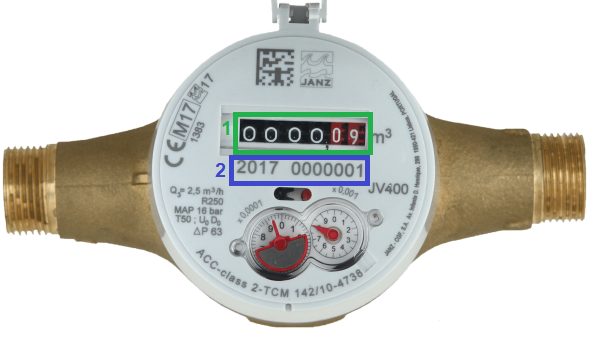
\includegraphics{diagramas/contador.png}}
\caption{Dispositivo indicador do contador de água.}
\label{fig:contador}
\end{center}
\end{figure}

\section{Sistemas Semelhantes} \label{sec:semelhantes}
Existem sistemas com funções e finalidades próximas ou até iguais ao sistema concebido. Deveremos analisar as várias funções destes sistemas, porém também as suas falhas e funcionalidades que deveriam ter sido implementadas, para que no nosso sistema possamos colmatar essas situações e oferecer uma solução mais competente e vantajosa.

\subsection{Aplicação para Dispositivo Móvel} \label{par:appsmas}
Os Serviços Municipalizados de Água e Saneamento de Almada e de Sintra já possuem, respetivamente, aplicações para \textit{smartphone} \cite{smas:almada} e websites \cite{smas:sintra} para as diferentes zonas em que operam. Estas plataformas permitem a gestão do contrato, consulta de contas, faturas e consumos, ativação de pagamento por débito direto, alteração de dados pessoais e a comunicação de leituras.\par
Comparando com o sistema Water Watcher, para além das funções que estes sistemas já possuem, o nosso sistema permite também aos utilizadores enviar as suas contagens através de uma fotografia do contador de água. Dado que o nosso sistema consegue reconhecer caracteres em imagens, futuramente, estaria mais preparado no caso de se instalarem dispositivos autónomos nos contadores que captam fotografias automaticamente, dado que apenas seria necessário que estes dispositivos enviassem as fotografias para o nosso sistema para que o processo de envio de contagens automáticas funcionasse corretamente.\par
O nosso sistema também permite o envio de contagens semanalmente, para que os clientes da empresa prestadora do serviço, caso estejam interessados, possam ter um controlo do seu consumo de água em períodos de tempo mais curtos, neste caso, semanalmente.

\subsection{Sistemas de Telemetria} \label{par:telemetria}
Existem, aplicados a esta área, sistemas de telemetria, ou seja, sistemas que efetuam a medição e comunicação das leituras. Alguns destes sistemas vêm incorporados no aparelho contador, existindo também outros que são um dispositivo separado \cite{janz:impji}. Porém, neste último caso, o contador de água tem de ser construído com características próprias que lhe permitam comunicar com estes dispositivos.\par
Nesta situação, no entanto, são necessárias estruturas intermediárias, como antenas, para mediar a comunicação entre o sistema informático da empresa e os sistemas de telemetria, dado que estes têm um alcance máximo de dez quilómetros em meio urbano \cite{mywater}. \par
Caso estes sistemas comunicassem com o Water Watcher, nomeadamente, através da aplicação móvel, não seriam necessárias estruturas intermediárias, nem alterações ao sistema excepto alterações para configurar esta nova comunicação.

\section{Progressive Web Apps} \label{sec:pwa}
Progresive Web Apps (PWA) ou aplicações web progressivas são aplicações que podem funcionar em qualquer dispositivo que possua um \textit{web browser}, sendo a principal característica que as define ser a junção das vantagens das aplicações web normais e das aplicações nativas, específicas para plataformas.\par
As aplicações web são aplicações que funcionam em qualquer dispositivo que suporte um \textit{web browser}, como computadores e \textit{smartphones}. Isto permite-nos ter uma base de código comum que funciona em vários dispositivos, ao contrário do que acontece com as aplicações nativas, o que resulta em construir e suportar menos código.\par
Porém, ao contrário das restantes aplicações web, as PWA permitem-nos utilizar funções específicas do dispositivo, como aceder à localização ou interagir com dados do dispositivo, tal como acontece com as aplicações nativas, ou seja, aplicações desenvolvidas especificamente para dispositivos com um mesmo sistema operativo, que consequentemente têm um conjunto de características semelhantes entre eles.

\section{Outsystems} \label{sec:outsystems}
Outsystems é uma plataforma que permite o desenvolvimento, testagem, implantação (ou \textit{deployment}) e monitorização de vários tipos de sistemas informáticos que utilizem aplicações móveis, aplicações web ou PWA.\par
É considerada uma ferramenta ‘low-code’, dado que gera automaticamente algum código que podemos utilizar no nosso projeto, o que ajuda no seu desenvolvimento e manutenção. Apesar de na licenciatura que frequentamos não tenha sido abordado o desenvolvimento de aplicações ‘low-code’, sentimos curiosidade em desenvolver o projeto segundo esta abordagem. Esta escolha foi motivada pelo facto de querermos estudar e colocar em prática conhecimentos sobre plataformas ‘low-code’, mas também para nos inteirarmos da plataforma Outsystems, dado que a nossa licenciatura nos dá conhecimentos para que possamos desenvolver a própria plataforma, que é desenvolvida em Portugal. \par
Segundo a análise da consultora Gartner \cite{gartner}, a Outsystems é uma empresa líder em plataformas de desenvolvimento de aplicações em ‘low-code’. Esta análise mostra que esta plataforma é das mais utilizadas neste contexto, o que foi um fator que influenciou positivamente a escolha desta plataforma para o desenvolvimento do sistema Water Watcher.\par
Esta plataforma também facilita a implantação (ou \textit{deployment}) do sistema informático. Ao compilar um módulo Outsystems, ele é publicado num \textit{workspace} privado ao utilizador. O \textit{workspace} é onde estão armazenados os módulos e extensões de cada utilizador. Quando um módulo é publicado, podemos aceder ao URI correspondente e aceder à aplicação cliente desses módulos, caso o módulo defina uma.\par
Este \textit{workspace} está alojado em estruturas computacionais geridas pela Outsystems, porém os sistemas informáticos desenvolvidos nesta plataforma são portáveis, na medida que é possível implantar o sistema em outras estruturas, como estruturas computacionais de outra empresa.\par
Nas subsecções \ref{sec:outsystemss} e \ref{sec:outsystemsi} vamos apresentar, respetivamente, o Outsystems Service Studio e o Outsystems Integration Studio, que são duas ferramentas da plataforma Outsystems que utilizamos para o desenvolvimento dos elementos do sistema informático desenvolvido no projeto.

\subsection{Outsystems Service Studio} \label{sec:outsystemss}
Outsystems Service Studio é uma ferramenta que nos permite desenvolver PWA. Esta ferramenta permite-nos desenvolver as várias componentes de um sistema informático, como a lógica do sistema, a sua componente visual de interação com o utilizador e o seu modelo de dados, o que é vantajoso, na medida em que apenas é necessário utilizar uma plataforma para a elaboração do sistema.\par
Por ser uma plataforma 'low-code', a forma de programar é diferente da que aprendemos e utilizamos durante licenciatura. Na figura \ref{fig:osjava} podemos comparar um excerto de código realizado na plataforma Outsystems Service Studio, com recurso à linguagem OML (Outsystems Markup Language), com um excerto de código numa linguagem abordada na licenciatura, neste caso, linguagem Java.

\vspace{5.5cm} 

\begin{figure}[ht!]
\centering
\resizebox{150mm}{!}{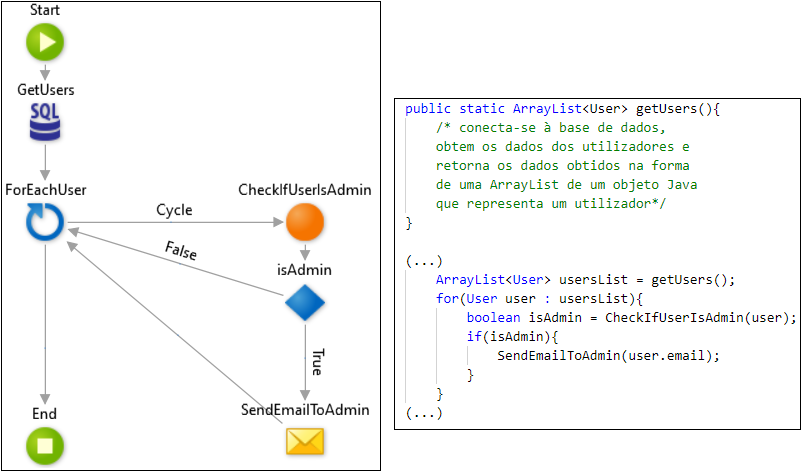
\includegraphics{diagramas/outs_vs_java.png}}
\caption{Comparação entre linguagem Outsystems e Java.}
\label{fig:osjava}
\end{figure}

Como podemos observar, a lógica de programação é semelhante em ambas as linguagens, porém podemos inferir algumas diferenças, como o facto de uma linguagem gráfica ser mais apelativa e fácil de ler e compreender, e não precisarmos de várias estruturas ou objetos diferentes para representar uma entidade, neste caso os utilizadores, o que é vantajoso na medida que não precisamos de ter preocupações com consistência e compatibilidade de tipos entre os vários atributos das estruturas. Na solução de código Java, para além da estrutura definida na linguagem utilizada na base de dados, é necessário uma outra estrutura (em Java denominada objeto) para representar um utilizador e os seus atributos. Na solução em código Outsystems utilizamos a mesma estrutura em todo o módulo para representar uma mesma entidade, o que é possível porque tanto o código utilizado para definir essa estrutura na base de dados como o código da lógica do sistema são desenvolvidos na mesma linguagem.\par
Outra vantagem do desenvolvimento de sistemas informáticos na plataforma Outsystems é não serem necessárias configurações ou desenvolver código para que os vários elementos de um sistema, como o sistema de gestão de bases de dados, a aplicação para os utilizadores e a aplicação servidora possam comunicar entre si.\par
Para além das vantagens referidas, a plataforma também facilita a construção de interfaces gráficas, oferecendo componentes, como listas, caixas de texto ou botões já definidas. Os componentes pretendidos podem ser simplesmente arrastados para uma tela que nos permite construir interfaces gráficas sem ser necessário escrever código.\par


\subsection{Outsystems Integration Studio} \label{sec:outsystemsi}
A ferramenta Outsystems Integration Studio possibilita o desenvolvimento de funções em linguagem de programação C\# que podem ser utilizadas no Outsystems Service Studio.\par
Com esta ferramenta podemos desenvolver extensões, que são equivalentes a classes nas linguagens de programação Java ou C\#, que contém funções. \par
Para definir uma função começamos por definir os seus parâmetros de entrada e de saída, mais concretamente, definir o seu nome e o seu tipo. O tipo dos parâmetros é escolhido de entre os vários tipos da plataforma Outsystems. Quando o código é gerado em C\#, o tipo selecionado anteriormente é transformado no seu tipo correspondente em C\# (por exemplo um parâmetro do tipo text será transformado no tipo String).\par
Após definir os parâmetros da função podemos editar o código C\# correspondente a essa função no editor Microsoft Visual Studio, podendo importar funções do sistema ou através de \textit{package managers} como o NuGet, adicionar novas classes e compilar o código.\par
Por fim, depois de definir as funções, podemos publicar a extensão gerada no nosso \textit{workspace} e utilizá-la nos módulos desenvolvidos no Service Studio.

\section{SysML} \label{sec:sysml}
A linguagem SysML(\textit{Systems Modeling Language}, normalizada no ISO/IEC 19514:2017\cite{isosys}) é uma linguagem de modelação desenvolvida principalmente para engenharia de sistemas. Esta linguagem é derivada da linguagem UML(\textit{Unified Modeling Language}), pelo que apresentam várias semelhanças nas notações e sintaxe utilizadas. \par
Para a elaboração dos diagramas nesta linguagem, utilizamos a ferramenta MagicDraw dado que, para além de nos permitir desenhar todos os diagramas que precisamos numa só ferramenta, de forma a manter consistência nas notações utilizadas, a empresa a quem pertence esta ferramenta fornece licenças de utilização aos estudantes do ISEL e a interface da ferramenta é semelhante à da interface da ferramenta Eclipse que utilizamos na licenciatura.\par
Neste relatório utilizamos Diagramas de Entidade Relação (\textit{Entity Relationship Diagrams}) para representar estruturas de dados e as relações entre elas. Utilizamos Diagramas Máquina de Estados SysML (\textit{SysML State Machine Diagrams}) para representar processos e ações sequenciais. Utilizamos também (\textit{SysML Block Definition Diagram}) para representar o sistema informático e os seus componentes. Por fim, para representar os requisitos do sistema e os seus casos de uso utilizamos, respetivamente, Diagramas de Casos de Uso SysML (\textit{SysML Use Case Diagrams}) e Diagramas de Requesitos (\textit{Requirement Diagrams}).

